% Audited version based on main_reframe_revised.tex; existing versions preserved.
\documentclass[letterpaper]{article} % DO NOT CHANGE THIS
\usepackage[submission]{aaai2027}  % DO NOT CHANGE THIS
\usepackage[hyphens]{url}  % DO NOT CHANGE THIS
\usepackage{graphicx} % DO NOT CHANGE THIS
\urlstyle{rm} % DO NOT CHANGE THIS
\def\UrlFont{\rm}  % DO NOT CHANGE THIS
\usepackage{natbib}  % DO NOT CHANGE THIS AND DO NOT ADD ANY OPTIONS TO IT
\usepackage{caption} % DO NOT CHANGE THIS AND DO NOT ADD ANY OPTIONS TO IT
\frenchspacing  % DO NOT CHANGE THIS
\usepackage{booktabs}
\usepackage{amsmath}
\usepackage{amssymb}

\pdfinfo{
/TemplateVersion (2027.1)
}

\setcounter{secnumdepth}{1} % the template allows 1 or 2

\newcommand{\fov}{\mathrm{FOV}}

\title{Equal Pixels, Unequal Views:\\Crop Field of View and Robust AI-Generated Image Detection}
\author{Anonymous Submission}
\affiliations{}

\begin{document}
\maketitle

\begin{abstract}
Fixed-size crops at native resolution preserve local image traces, but their
field of view shrinks as image size increases. We study how this
preprocessing choice affects AI-generated image detection under degradation,
distinguishing each crop's field of view from the total image area covered
by multiple crops. With frozen, crop-trained DINOv2 detectors, replacing a
central crop with a resized whole image raises robust ROC AUC from 0.886 to
0.963 on the NTIRE 2026 hard validation split used for policy selection. On
large held-out SocialRF images with synthetic degradations, whole-image
input improves AUC by 7.9--9.1 AUC points. Factorial experiments show
that downscaling before cropping benefits DINOv2, CLIP, and B-Free on this
benchmark, while increasing coverage from 25\% to 100\% of image area at fixed scale provides little additional gain on degraded SocialRF. Resizing controls support a role for wider per-crop context,
although interpolation and changes in crop count limit causal attribution.
A separately trained whole-image system improves NTIRE test robust AUC by
0.062 while reducing clean AUC by 0.014. Benefits therefore depend on the
detector, dataset, and degradation. We additionally identify format and size
confounds in two evaluated benchmark configurations. These findings motivate
reporting crop field of view and resize factors alongside detector input
resolution.
\end{abstract}

\section{Introduction}
\label{sec:intro}

Deployed detectors of AI-generated images see what social platforms deliver:
images that have been recompressed, resized and filtered, at every size. A
detector must turn each one into a fixed-size input. Forensic work recommends avoiding resizing because interpolation can erase subtle high-frequency generation traces
\cite{corvi2023detection}. The usual answer is a fixed-size crop at native
resolution, which we call a \emph{window}, scored once or several times with
the scores averaged
\cite{corvi2023detection,li2025safe,guillaro2025bfree,konstantinidou2025texturecrop}.

A fixed input resolution does not fix how much of the source image a
detector observes. We call each square input a \emph{view}, and define a
crop's field of view as its side length $s$ divided by the source image's
short side $h$: $\fov = s/h$. A 200-pixel crop spans 39\% of a 512-pixel
image's short side but only 5\% of a 4000-pixel image's. Scoring additional
native crops increases total image \emph{coverage} while retaining this
narrow field of view in each input. Downscaling before cropping instead
widens each input's field of view, while also changing resampling and
aggregation. Which aspects of input presentation account for robustness
gains on degraded images?

We investigate this question using detectors trained for the NTIRE 2026
Robust AI-Generated Image Detection challenge \cite{gushchin2026ntire}.
All 407k training images have a short side of at most 512 pixels.
Augmentation changes the field of view, but no sampled training view spans
less than approximately 20\% of the short side. On the hard validation
split, a native window can span only 5\%, and robust AUC falls as image
size grows. Presenting the whole image to the frozen crop-trained models
improves robust AUC by 7 to 9 points per branch. We examine this effect
through controlled changes to coverage and downscale factor, and evaluate
its transfer and clean-image cost on held-out data.

\paragraph{Contributions.}
\begin{itemize}
\item \textbf{Preprocessing diagnosis.} Whole-image presentation substantially
  improves robust AUC for frozen, crop-trained DINOv2 detectors, exceeding
  the gain from averaging nine native crops while requiring only one view
  (Sec.~\ref{sec:diagnosis}).
\item \textbf{Controlled analysis.} We vary coverage and downscale factor
  independently within a tiled protocol and use resizing controls to
  examine competing explanations. On degraded SocialRF, downscaling
  benefits DINOv2, CLIP, and B-Free, while additional coverage contributes
  little between 25\% and 100\% of image area (Secs.~\ref{sec:controls}, \ref{sec:decomp}, and \ref{sec:heldout}).
\item \textbf{Transfer and limitations.} We report external evaluations, a
  declared second NTIRE test evaluation, clean-image losses, and
  unsuccessful comparisons. We also identify format and size confounds in
  the evaluated CommunityAI and Synthbuster/RAISE configurations
  (Secs.~\ref{sec:heldout} and \ref{sec:leaks}).
\end{itemize}

Whole-image resizing already appears in detection pipelines. The NTIRE
2026 winner resizes at inference to preserve global spatial context, the
fifth-placed team uses \emph{squish} \cite{gushchin2026ntire}, and AI-GenBench
\cite{pellegrini2025aigenbench} finds resizing often preferable to multi-crop
evaluation for CLIP and DINOv2. We investigate the explanations behind these
observations by varying per-crop field of view and total coverage, and by
testing resizing controls. The contribution is an empirical analysis of
when these choices help and where they fail.

\section{Related work}
\label{sec:related}

\paragraph{Historical context.} Random crops and multi-crop inference long predate image forensics \cite{krizhevsky2012imagenet}; random resized crops vary apparent object scale \cite{szegedy2015going}. For generated-image detection, blur and JPEG augmentation already improve transfer \cite{wang2020cnn}. Our contribution is an empirical comparison of crop field of view, coverage, and resizing under degradation, not a new resize operator.

\paragraph{Crop, don't resize.} Native-patch scoring and fusion preserve local traces \cite{corvi2023detection}. SAFE replaces downsampling with crops \cite{li2025safe}; B-Free trains on 504-pixel crops and averages native windows \cite{guillaro2025bfree}; SPAI scores arbitrary resolutions spectrally \cite{karageorgiou2025spai}; TextureCrop selects textured native windows \cite{konstantinidou2025texturecrop}. HiDA-Net combines native tiles and a global view \cite{mu2026hidanet}. These motivate preserving local traces, but do not establish that crops always win under degradation. SAFE's CNN performs similarly with center crops and full native images in its ablation, limiting extrapolation across detector families.

\paragraph{Resize can win.} AI-GenBench reports resize versus five-crop AUROC of 94.24 versus 93.44 for fine-tuned DINOv2, and 92.04 versus 87.66 for CLIP \cite{pellegrini2025aigenbench}. AIGIBench's CLIP detector favors resize while five low-level detectors favor crops \cite{li2025aigibench}. Other pipelines resize before cropping \cite{cozzolino2024raising} or tiling \cite{choi2025warpad}. GlobalForge's clean GenImage experiment gives crop-trained UnivFD 67.90 balanced accuracy under crops versus 58.70 under resize; its resize-trained model instead scores 67.50 with resize and 67.10 with crops (Fig.~2) \cite{cui2026globalforge}. These balanced accuracies on another dataset are not directly comparable to our AUCs.

\paragraph{Scale and size as confounds.} JPEG quality and image size can separate labels, and cropping retains object-scale bias \cite{grommelt2024fakeorjpeg}. Random resized crops introduce resampling signals when class sizes differ \cite{rajan2025aligned}; BIAS-ID measures transformation-induced score shifts \cite{ricker2026biasid}. FixRes studies train-test apparent-scale discrepancies \cite{touvron2019fixres}. We examine per-crop field of view while retaining content scale and resampling as alternative explanations.

\section{Setup}
\label{sec:setup}

\begin{figure*}[t]
\centering
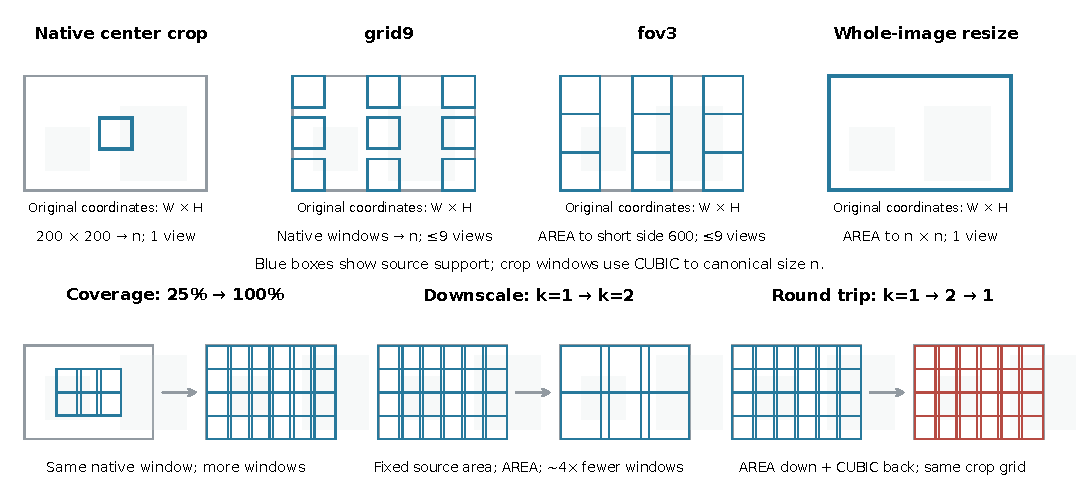
\includegraphics[width=\textwidth]{fig_preprocessing_audited.pdf}
\caption{Preprocessing interventions. Top: views marked in original-image coordinates; $n$ is the canonical input size (512 for A, 224 for B). FOV and coverage differ even with equal input pixels. Below: coverage changes at fixed native scale; downscaling at fixed source coverage widens each view and reduces the number of windows; a round trip restores the original crop grid with additional interpolation. Counts are illustrative; duplicate positions are removed. Branch A additionally resizes 512 to 518 before its tower.}
\label{fig:preprocessing}
\end{figure*}

\paragraph{Data.} We train on 407,223 images: the NTIRE 2026 training shards,
COCO \cite{lin2014coco} and Open Images \cite{kuznetsova2020openimages} reals, and paired real and generated images from several
open and commercial generators. Every training image has a short side of 200 to
512 pixels (median 512, and 384 or more for 95\% of images). We evaluate on the organizers' labeled splits:
\texttt{ntire\_val} (10,000 images, half distorted), \texttt{ntire\_val\_hard}
(2,500, half distorted) and the public test split \texttt{ntire\_test}
(2,500, half distorted). Robust AUC is the ROC AUC over distorted images, and clean AUC is
over undistorted ones, following the challenge \cite{gushchin2026ntire}.

\paragraph{Why 200 pixels?} The crop policy originated in an earlier benchmark configuration whose real images had a 200-pixel information ceiling; 200 was also the minimum short side in this training set. A native window avoided reducing larger images to that ceiling while standardizing their pixel count. This historical choice is not an optimality claim. Native-224, native-512, and 196-pixel controls test its sensitivity (Sec.~\ref{sec:training}; supplement S10).

\paragraph{Models.} Both branches fine-tune all 24 blocks of DINOv2-L/14 with registers \cite{oquab2024dinov2,darcet2024registers}, with mean-pooled patch tokens (0.91B parameters total). A uses one tower, 512-pixel canonicalization and a 518-pixel tower input, for two epochs; B concatenates two 224-pixel towers for three epochs. The bank supplies ten degraded candidates per source; each training draw samples one clean and two degraded views. Recipes chain up to five of 26 operations in six families, including a neural codec \cite{balle2018hyperprior} and pre-crop downscaling. Loss combines class-balanced cross-entropy, degradation prediction (0.3), and output/feature consistency (unit weights). Cosine scheduling uses 3\% warm-up and weight averaging over the final quarter \cite{izmailov2018swa}. Supplement S3 documents sampling and kernels.

\paragraph{Views, field of view and coverage.} A \emph{view} is one
square input to the model: a region of the image resized to the branch's input
size. A detector may score several views of one image and average their
logits. The \emph{field of view} of a view is the share of the image's short
side it shows. \emph{Coverage} is the share of the image area that all views
of one image show together. A 200-pixel window cut after the image is
downscaled by a factor $k$ has $\fov = 200k/h$, provided the window fits.
For a fixed-size window, downscaling widens its field of view and increases
the source area it covers. In our fully tiled construction below, total
coverage is held fixed while the downscale factor varies.

The \emph{crop} policy takes one 200-pixel window at native resolution (the
center window at test time) and resizes it to the branch's input size. Images
with a short side under 200 pixels are taken whole. The \emph{squish} policy
resizes the whole image to the input size, discarding aspect ratio: area
interpolation on the short side down to the input size when the image is
larger, then area interpolation to the square. Both policies give every image
the same number of input pixels. Under squish, field of view and coverage are
both 1. To vary the two one at a time, \emph{tiles}$(k, f)$ takes the centerd
region holding a fraction $f$ of the image area, downscales it by $k$ with
area interpolation, covers it with 200-pixel windows, resizes each window to
the input size and averages the logits. $f$ sets coverage and $k$ sets each
view's field of view. Downscaling also changes interpolation and the
number of windows averaged, so these are experimental contrasts rather
than isolated causal effects.



\paragraph{Comparison types.} Frozen-model comparisons change presentation
at test time while retaining branch checkpoints. Training comparisons use
separately crop-trained and squish-trained models. The final test read
compares complete systems, including their checkpoints and fitted fusion
settings. We distinguish these throughout.

\paragraph{Fusion and selection.} The two branches' logits are z-scored and
combined as $w z_A + (1-w) z_B$. For each configuration, logit mean and population SD are estimated on its fit rows; these are separate from weight selection, which maximizes mean robust and clean AUC over $w=0,0.05,\ldots,1$. Table~\ref{tab:fusion} distinguishes the configurations. Squish final/SWA checkpoint selection uses \texttt{ntire\_val}; crop retains the earlier choice from both validation splits. A later validation-only check gives the same crop picks (A final, B SWA).

\begin{table}[t]
\centering\small
\begin{tabular}{lcl}
\toprule
configuration & $w$ & fit splits \\
\midrule
crop, validation/external & 0.50 & val \\
frozen crop, whole-image input & 0.50 & val \\
trained whole-image input & 0.55 & val \\
historical crop, test read 1 & 0.45 & val + hard \\
\bottomrule
\end{tabular}
\caption{Fusion configurations. ``val'' and ``hard'' abbreviate the two NTIRE validation splits. Both z-score estimation and weight selection use the listed fit population, with separately estimated statistics for each configuration.}
\label{tab:fusion}
\end{table}

\paragraph{Statistics.} All intervals are 95\% percentile intervals from 2,000
paired bootstrap resamples, stratified by label and distortion status (or label within a fixed-status subgroup), with the same indices within a comparison. Intervals are unadjusted for multiple comparisons. One AUC point is 0.01 AUC. Differences without a saved paired interval are point estimates. Pooled AUC ranks all real/fake pairs together, not an average over generators. TPR at 1\% FPR uses the lowest empirical threshold with FPR $\leq0.01$ on the same reported population; it is a retrospective ROC operating point, not a threshold frozen for deployment.

\paragraph{Protocol.} The test split was first read with the crop fusion
(2026-10-04). A registration describes one further test read, reported as 2026-10-11 16:45 UTC. Its initial text is verifiable in an October 8 commit. Later amendments have weaker timing provenance: amendments 7--12 first appear in the available history on November 2, despite earlier dates in their text. We distinguish declared protocols from independently verified pre-run ordering (supplement S13). A third read was conditionally planned for routed fusion and subsequently canceled; no third read is reported. This audit uses only saved reports and runs no model evaluation. We chose squish on \texttt{ntire\_val\_hard}, the \emph{selection split}; external data and the declared second test read provide evidence beyond selection. Anonymized declarations accompany the supplement; code and scores are intended for later release.

\section{Equal pixels, unequal views}
\label{sec:diagnosis}

\begin{table}[t]
\centering
\small
\begin{tabular}{lrrrr}
\toprule
split & n & p5 & p50 & p95 \\
\midrule
train, native & 407,223 & 0.391 & 0.391 & 0.521 \\
train, window taken & 220,000 & 0.391 & 0.468 & 1.000 \\
train, after second crop & 220,000 & 0.296 & 0.415 & 0.942 \\
\texttt{ntire\_val} & 10,000 & 0.100 & 0.312 & 0.893 \\
\texttt{ntire\_val\_hard} & 2,500 & 0.112 & 0.298 & 0.784 \\
\bottomrule
\end{tabular}
\caption{Field of view ($200/$short side). Training estimates use 20,000 seeded images with 11 candidate views each. Pre-window downscaling widens views; a later crop can narrow them to 0.195. On hard validation, 70.8\% of views are below 0.391 and the minimum is 0.05. Candidate-view analysis differs from actual training draws (supplement S3).}

\label{tab:fov}
\end{table}

Table~\ref{tab:fov} shows how much of each image the window covers. The
central 90\% of native training field-of-view values lie between 39 and
52\% of the short side. Augmentation widens some views and narrows others;
the minimum observed after the second crop is approximately 20\%. On \texttt{ntire\_val\_hard} the median
is 30\%, and one image in twenty gets 11\% or less. Under the crop policy,
fused robust AUC on \texttt{ntire\_val\_hard} falls from 0.911 for images
with a short side of 80 to 336 pixels to 0.865 for images above 752 pixels.
The trained-system size comparison appears separately in Sec.~\ref{sec:training}.



\begin{figure*}[t]
\centering
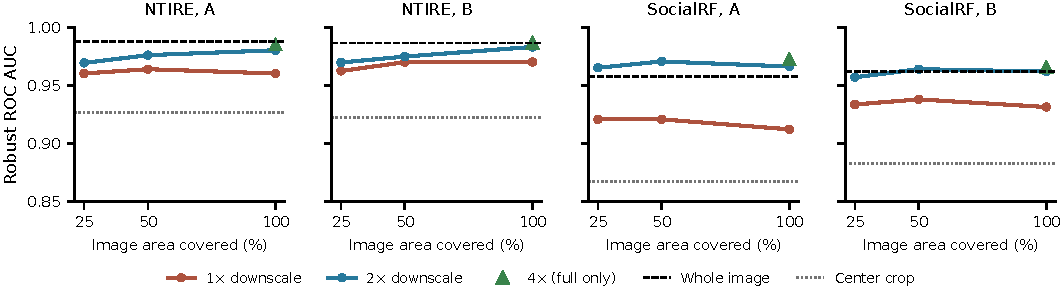
\includegraphics[width=\textwidth]{fig_tiles_audited.pdf}
\caption{Robust AUC of \emph{tiles}$(k, f)$ for the frozen crop-trained
branches on images with a short side of at least 800 pixels. Moving right
tiles more of the image with same-size windows (coverage). Different lines vary the downscale factor, also changing field of view
and window count. NTIRE pools both validation splits. On held-out SocialRF,
coverage from 25\% to 100\% of image area contributes little additional gain under our degradation chains; the initial single-crop-to-quarter gain is excluded from this contrast. Dashed: squish. Dotted: the
center window.}
\label{fig:tiles}
\end{figure*}

To test whether additional native crops recover the gain, we scored the two frozen
crop-trained branches under four test-time presentations
(Table~\ref{tab:probe}). \emph{grid9} averages nine 200-pixel native windows,
nine times the pixels at the same field of view. \emph{fov3} first downscales
the short side to 600 pixels and then takes the nine windows, which sets the
field of view to $1/3$ when the short side exceeds 600; smaller images retain native scale. Duplicate window coordinates are removed. \emph{squish} shows the whole image once.

\begin{table}[t]
\centering
\small
\setlength{\tabcolsep}{4pt}
\begin{tabular}{llrrr}
\toprule
branch & presentation & views & robust & clean \\
\midrule
A (512) & center window & 1 & 0.8561 & 0.9912 \\
        & grid9 & 8.9 & 0.8495 & 0.9978 \\
        & fov3 & 8.9 & 0.8703 & 0.9977 \\
        & squish & 1 & \textbf{0.9482} & 0.9906 \\
\midrule
B (224) & center window & 1 & 0.8872 & 0.9801 \\
        & grid9 & 8.9 & 0.9049 & 0.9931 \\
        & fov3 & 8.9 & 0.9215 & 0.9942 \\
        & squish & 1 & \textbf{0.9599} & 0.9886 \\
\bottomrule
\end{tabular}
\caption{Frozen crop-trained branches under four test-time presentations
on the hard validation split (selection split). Averaging additional native windows
(grid9) helps B by 1.8 points and costs A 0.7. Whole-image input gives
the largest robust AUC for both branches.}
\label{tab:probe}
\end{table}

Additional native windows yield smaller changes than whole-image input: grid9 gains 1.8 robust
points on B and loses 0.7 on A. The intermediate fov3 presentation gains 1.4
and 3.4 points, and squish gains 9.2 and 7.3. Squish uses one view and the
same pixel count as the center window. On B the paired interval for the
squish gain is [+0.057, +0.090]. With z-scores and weight fitted on
\texttt{ntire\_val}, the fused robust AUC rises from 0.886 to 0.963 and the
pooled true positive rate at 1\% false positive rate from 0.516 to 0.752. Clean AUC
moves by $-0.001$ on A and $+0.009$ on B.

Squish changes three things at once. It raises coverage to the whole
image, widens the field of view of its one view, and resamples local image
traces and degradations. Figure~\ref{fig:tiles} previews the coverage/downscale contrasts of
Sec.~\ref{sec:decomp}, following controls for resolution cues and aspect ratio.



\section{Controls for resolution and aspect ratio}
\label{sec:controls}

Resizing can leave cues about native resolution: small images are enlarged
and large images reduced. Four controls test whether such cues explain the
gain. First, native short side has a monotone size-label AUC of 0.528 in
training. This weakens a simple size-shortcut account but does not exclude
nonlinear cues. Second, within native-size deciles (branch B only; no saved branch-A decile result), where resize factors
vary less, squish beats the center window in all ten deciles on branch B
(size-weighted robust AUC 0.888 to 0.964). Third, band-limiting the squished
input to 160 pixels reduces available resolution cues, yet B retains +7.2
of its +7.3 points and A retains +5.7 of +9.2. This control also removes
image detail and cannot guarantee that all size cues disappear. Fourth,
on rows with only photometric transforms (median short side 784 pixels),
the gain is +9.0 points on A and +8.3 on B, with intervals above zero.
The effect therefore does not require the challenge's geometric
transforms \cite{gushchin2026ntire}.

Squish also stretches non-square images, potentially introducing frequency
artifacts along one axis \cite{grommelt2024fakeorjpeg}. Two
aspect-preserving presentations, a center square after resizing the short
side and a padded letterbox, retain 93 to 100\% of its robust gain.
Aspect-ratio distortion is therefore unnecessary for most of the measured
improvement.

\section{Coverage and downscale contrasts}
\label{sec:decomp}

This section uses frozen crop-trained checkpoints throughout. The NTIRE
analyses pool both validation splits; SocialRF provides external data with
our synthetic degradation chains.

\paragraph{Degradation and size.} We took the 6,250 undistorted images of the
two validation splits and applied JPEG (quality 90, 70, 30), Gaussian blur
($\sigma$ 0.5, 1, 2) or Gaussian noise ($\sigma$ 0.02, 0.05, 0.10) at native
resolution. The robust gain of squish over the center window, averaged over
the three operations, rises from $-0.001$ with no degradation to $+0.029$ at
the heaviest level on branch A, and from $+0.004$ to $+0.027$ on B. Every
rise from none to heavy has an interval above zero, pooled and in every size
bucket. The rise is largest above 752 pixels ($+0.049$ on both branches). On
undistorted images up to 736 pixels the two policies differ by at most
0.002. The levels are not matched in strength across operations, so we do
not rank the operations.

\paragraph{Coverage against downscale.} The images used here have a short
side of at least 800 pixels. We scored \emph{tiles}$(k, f)$ at
$k \in \{1, 2\}$ and $f \in \{0.25, 0.5, 1\}$, so every window is a
200-pixel window like those in training. A 4$\times$ condition is evaluated only at full coverage, outside this $2\times3$ factorial. The coverage effect $d_F$ is the
gain from $f = 0.25$ to $f = 1$ averaged over $k$. The downscale effect $d_K$
is the gain from $k = 1$ to $k = 2$ averaged over $f$. On NTIRE (4,068 images,
1,235 distorted, pooled validation splits) both effects are above zero on both branches
(Table~\ref{tab:decomp}). On large degraded SocialRF images, which no model
was trained or selected on, increasing coverage from 25\% to 100\% of image area provides little additional gain: at a fixed downscale,
showing the whole image instead of its central quarter changes robust AUC by
less than 0.01. The downscale helps by 2.3 to 5.5 points at every coverage
level, more than on NTIRE. Covering the whole image after a 4x downscale,
\emph{tiles}$(4, 1)$, is within 0.003 of squish on NTIRE and at least as good
on SocialRF (A 0.973 against 0.958, B 0.966 against 0.962).
The exact frozen-branch SocialRF center-to-whole-image values are A $0.867656\to0.958200$ and B $0.882892\to0.962304$: +9.1 and +7.9 AUC points. These are point-estimate differences on 1,000 degraded images (500 per class; 2,000 rows including clean counterparts), not trained-fusion or B-Free results. Native tiling of just the central quarter already gains 5.34 points on A and 5.10 on B over one center crop (point estimates without saved paired intervals). Thus our weak additional-coverage result concerns 25--100\% area, not one crop versus many crops.
Figure~\ref{fig:tiles} shows the stronger downscale effect on SocialRF,
where the coverage curves are comparatively flat.

\paragraph{Round-trip resizing control.} Round-trip resizing tests whether
downscaling helps when each crop retains its original field of view. We
downscale each region by two, restore its dimensions, and evaluate the
original crop grid. Let $d_A$ be the AUC difference between this round trip
and \emph{tiles}$(1,f)$, averaged over $f$, and let $d_V=d_K-d_A$ be the
residual contrast against \emph{tiles}$(2,f)$. These are the
\emph{round-trip resize effect} and \emph{residual downscale effect},
respectively. For DINOv2, $d_A$ is at most approximately 0.004 in magnitude on both
datasets and branches, with intervals including zero; the residual
contrast is positive (Table~\ref{tab:decomp}). This pattern is consistent
with a benefit from wider per-crop context, but does not establish
equivalence or identify a pure field-of-view effect. The round trip adds
interpolation, and directly downscaled inputs average about four times
fewer windows. These changes can affect both detail retention and pooling.

\paragraph{Stronger downscales.} A separate ordering control uses 2,833 originally undistorted NTIRE validation images with short side $\geq800$ (1,520 real, 1,313 fake), applying heavy JPEG, blur, or noise before versus after downscaling. $R(k)$ averages the three operation-specific before-minus-after AUC differences. A gives $R(2)=+0.022$ [0.019, 0.026] and $R(4)=+0.036$ [0.032, 0.041]; B gives +0.007 [0.005, 0.008] and +0.013 [0.010, 0.015]. The ordering effect grows at 4$\times$, consistent with attenuation, but effective degradation scale also changes. This is a different population and contrast from the factorial; supplement S9 reports the details.

\paragraph{Possible mismatch in each view.} No sampled training view spans
less than approximately 20\% of the short side, while a 200-pixel crop of a
3,000-pixel photo spans 7\%. Downscaling moves its field of view toward the
observed training range, consistent with a train-test mismatch related to
the scale discrepancy studied by FixRes \cite{touvron2019fixres}.
However, frozen models also gain within the native training-size band: among 171 distorted selection-split images with short sides 416--496 pixels (86 real, 85 fake), whole-image input gains +11.1 [5.9, 17.0] AUC points on A and +7.9 [3.6, 12.9] on B. Training-size mismatch alone cannot explain the results. Wider context remains an interpretation because content scale and resampling change too.

\paragraph{CLIP.} We repeat the contrasts on three short crop-trained CLIP
ViT-L/14 runs (Sec.~\ref{sec:training}) using the same SocialRF images.
Downscaling improves robust AUC by 5.4 to 7.6 points, while increasing coverage from 25\% to 100\% of image area provides little additional gain on degraded SocialRF. The residual contrast $d_V$
is +0.041 to +0.063. The round-trip effect $d_A$ is also positive:
+0.011 to +0.014 on degraded images, with intervals above zero on all
seeds. However, it improves clean AUC by +0.022 to +0.025 as well.
The round-trip benefit therefore cannot be attributed specifically to
degradation removal.

\begin{table}[t]
\centering
\footnotesize
\setlength{\tabcolsep}{4pt}
\begin{tabular}{llrrrr}
\toprule
data & branch & $d_F$ & $d_K$ & $d_A$ & $d_V$ \\
\midrule
NTIRE & A & +0.005* & +0.014* & $-0.002$ & +0.016* \\
      & B & +0.011* & +0.008* & $-0.001$ & +0.010* \\
SocialRF & A & $-0.004$ & +0.050* & +0.001 & +0.049* \\
         & B & +0.001 & +0.027* & +0.004 & +0.023* \\
\bottomrule
\end{tabular}
\caption{Robust-AUC contrasts for frozen crop-trained branches,
images with a short side of at least 800 pixels. $d_F$: coverage, from 25\% to 100\% of the image. $d_K$: downscale by 2.
$d_A$: round-trip resize effect. $d_V$: residual downscale effect
($d_A+d_V=d_K$); neither is an isolated causal component. NTIRE rows pool both validation splits. SocialRF rows
use our degradation chains. * marks a 95\% interval that excludes zero.}
\label{tab:decomp}
\end{table}



\section{Training and baselines}
\label{sec:training}

\begin{figure}[t]
\centering
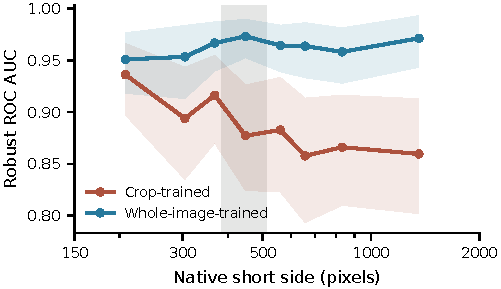
\includegraphics[width=\columnwidth]{fig_size_audited.pdf}
\caption{Fused robust AUC on the distorted rows of \texttt{ntire\_val\_hard}
(selection split) in eight equal-count bins of native short side, with 95\%
bootstrap bands. Red: the crop-trained fusion under its 200-pixel window.
Blue: the separately squish-trained fusion. This is a comparison of
trained systems, not the frozen-checkpoint intervention in
Table~\ref{tab:probe}. Grey: the 384--512-pixel band containing at least
95\% of native training short sides.}
\label{fig:size}
\end{figure}

\paragraph{Training under whole-image input.} In short training runs (one tower,
one epoch on a quarter of the training set, three seeds), squish-trained
models beat crop-trained ones by +0.083 [+0.062, +0.105], +0.093 [+0.072,
+0.115] and +0.078 [+0.057, +0.102] robust AUC on \texttt{ntire\_val\_hard},
with clean AUC within noise. We then trained the full branches under squish
(Table~\ref{tab:branches}). Their robust AUC is close to that of the frozen test-time intervention (A:
0.943 against 0.948, B: 0.959 against 0.960), with slightly higher clean AUC. The
fused squish-trained models reach 0.960 robust and 0.995 clean, against 0.886
and 0.990 for the crop fusion: +0.074 [+0.058, +0.091]. Across the eight bins of Figure~\ref{fig:size}, the whole-image-trained fusion stays between 0.951 and 0.973. In the short runs, training under squish adds 4 to 6
points beyond the test-time change, with DINOv2 and with CLIP (an
exploratory comparison). The full branches show no such gap. They
differ from the short runs in training length, number of views per image and
loss terms, and we cannot say which of these closes the gap.

\begin{table}[t]
\centering
\small
\setlength{\tabcolsep}{4pt}
\begin{tabular}{llcc}
\toprule
branch & model & robust & clean \\
\midrule
A & crop-trained & 0.8561 & 0.9913 \\
  & crop-trained, squish at test & 0.9482 & 0.9906 \\
  & squish-trained & 0.9425 & 0.9934 \\
\midrule
B & crop-trained & 0.8873 & 0.9801 \\
  & crop-trained, squish at test & 0.9599 & 0.9886 \\
  & squish-trained & 0.9589 & 0.9898 \\
\bottomrule
\end{tabular}
\caption{Per branch on \texttt{ntire\_val\_hard} (selection split). Training under
squish yields similar point estimates to presenting the whole image to
the frozen crop-trained model; this is not an equivalence test. Paired gains over crop-trained: A +0.092 and +0.086, B
+0.073 and +0.072, all intervals clear of zero. The crop-trained rows were
rescored for this table and differ from Table~\ref{tab:probe} by at most 0.0001; the source of this cross-pass drift is not documented (supplement S12).}
\label{tab:branches}
\end{table}

\paragraph{A second backbone.} We repeated the short-run comparison with a CLIP
ViT-L/14 tower \cite{radford2021clip} in place of DINOv2, every other setting
unchanged. Over three seeds, training under squish beat crop by +0.139 to
+0.150 robust AUC, with clean AUC near the crop baseline, and showing the crop-trained
checkpoints the whole image gained +0.094 to +0.111 at test time alone, every
interval clear of zero. Both gains grow with size: at test time, +0.168 above
752 pixels against +0.057 below 336. CLIP's crop-trained short runs are weaker
than DINOv2's (0.748 robust against 0.799) and gain more.

\paragraph{Sensitivity to crop size and aggregation.} Branch A enlarges 200 to 512 during canonicalization (2.56$\times$), then to the 518-pixel tower input (2.59$\times$ overall); B enlarges 200 to 224 (1.12$\times$). Native-224 proxies retain a mean 7.7-point gap to whole-image training. A single-seed native-512 proxy improves robust AUC, but changes field of view as well as enlargement. On exactly 630 distorted selection-split images with short side $\geq512$, the native-512 minus enlarged-200 contrast is +0.059 [0.032, 0.087]; native-512 minus native-196 is +0.048 [0.022, 0.072]; native-196 minus enlarged-200 is +0.011 [$-0.014$, +0.037]. These do not isolate interpolation: the small window changes by 2\%, patch-token count changes nearly sevenfold, and pixel-scale augmentation differs. Native-512 also receives a 512-to-518 resize. Supplement S10 gives populations, clean costs, and native-crop details.

Multi-scale training closes 73--81\% of the crop-to-whole-image gap, with whole-image input still ahead by 1.9 points on average. A validation-fitted attention combiner improves nine-crop averaging by about 3 points, yet frozen whole-image input remains ahead by +0.069 [0.052, 0.087] on A and +0.023 [0.011, 0.036] on B (supplement S11). No one control isolates a pure field-of-view effect.

\section{Held-out evidence and where it stops}
\label{sec:heldout}

\paragraph{External benchmarks.} We compare separately trained crop and
squish fusions on three external benchmarks that no model was trained or selected on, after removing any image whose content
digest matched an NTIRE image: AIGIBench SocialRF and CommunityAI
\cite{li2025aigibench}, and Synthbuster with RAISE-1k reals
\cite{bammey2024synthbuster,dangnguyen2015raise}. All three have no added degradation in their distributed form, so we
report pooled AUC on the files as distributed, on every file re-encoded as
JPEG at quality 95, and on every file passed through one seeded chain from
our degradation pool. That last reading is our own synthesis, not the
organizers'.

\begin{table*}[t]
\centering
\small
\begin{tabular}{lccc}
\toprule
 & SocialRF & CommunityAI & Synthbuster \\
\midrule
n (real/fake) & 2994/3000 & 6000/6000 & 994/8996 \\
short side p50 & 1366 & 500 & 833 \\
size-label AUC & 0.694 & 0.916 & 0.519 \\
format-label AUC & 0.500 & 1.000 & 0.555 \\
\midrule
crop fusion & 0.9633 & 0.9809 & 0.9995 \\
squish fusion & 0.9776 & 0.9920 & 0.9984 \\
difference & +0.014 & +0.011 & $-0.001$ \\
\quad 95\% CI & [+0.010, +0.018] & [+0.009, +0.013] & [$-0.002$, $-0.001$] \\
\midrule
size-matched, JPEG 95 & +0.016 & +0.005 & n/a \\
\quad 95\% CI & [+0.009, +0.024] & [$-0.002$, +0.012] & \\
JPEG 95, crop / squish & 0.9653 / 0.9778 & 0.9802 / 0.9920 & 0.9993 / 0.9986 \\
\quad difference [95\% CI] & +0.0126 [0.0084, 0.0166] & +0.0118 [0.0098, 0.0139] & $-0.0008$ [$-0.0014$, $-0.0002$] \\
degraded (ours), difference & +0.085 & +0.070 & +0.024 \\
\quad 95\% CI & [0.077, 0.092] & [0.065, 0.075] & [0.020, 0.028] \\
\bottomrule
\end{tabular}
\caption{External benchmarks, separately trained crop and squish fusions.
Size-matched is the size-weighted AUC within native-size deciles containing
both classes (all 5,994 SocialRF images; 5,920 of 12,000 CommunityAI images). It cannot be computed on Synthbuster
because no decile holds both classes (Sec.~\ref{sec:leaks}). Intervals use saved paired differences; supplement S12 reconciles repeated values across the saved reports.}
\label{tab:external}
\end{table*}

Table~\ref{tab:external} gives the results. On SocialRF, squish has higher AUC on the files as distributed, after JPEG re-encoding, and within size deciles, and on
its large degraded images the frozen-model contrasts favor downscaling
(Sec.~\ref{sec:decomp}). On CommunityAI the pooled gain is confounded: every
real image is a JPEG and every fake a PNG, and native size alone separates
the classes with AUC 0.916. The size-matched gain on the re-encoded files does
not clear zero ([$-0.002$, +0.012]). On Synthbuster squish loses by 0.001,
with both fusions near ceiling. Under our degradation chains squish wins on
all three sets, by 2.4 to 8.5 points. Higher AUC does not ensure a better strict operating point: on SocialRF as distributed, TPR at 1\% FPR is 0.538 for crop versus 0.482 for whole-image input; after JPEG 95 it is 0.560 versus 0.490. These TPR differences are point estimates without saved intervals.

\paragraph{The second test read.} Table~\ref{tab:test} gives both reads of
the public test split. Read 1 used the crop fusion as frozen on 2026-09-23.
Read 1 was evaluated October 4; its September 23 date is the configuration freeze date. Read 2 was evaluated October 11 after its validation fit; an exact independent freeze timestamp is unavailable. No third test evaluation was performed. Robust AUC changed by +0.062 [+0.040, +0.083] and clean AUC by $-0.014$ [$-0.024$, $-0.006$]. These are complete-system
differences, including training, checkpoint selection, and fusion settings;
they do not isolate a frozen-model preprocessing effect. \begin{table}[t]
\centering
\small
\begin{tabular}{lcccc}
\toprule
read/system & robust & clean & AUC & TPR@1\% \\
\midrule
1, crop & 0.7931 & 0.9856 & 0.9108 & 0.289 \\
2, squish & 0.8547 & 0.9715 & 0.9211 & 0.300 \\
\bottomrule
\end{tabular}
\caption{Complete-system comparison on \texttt{ntire\_test} (2,500 images).
The two reads use different trained checkpoints. TPR is pooled and uses a retrospective ROC threshold on the scored reals. Read 1's fusion
weight was fitted on both validation splits ($w = 0.45$), read 2's on
\texttt{ntire\_val} alone.}
\label{tab:test}
\end{table}

\paragraph{The clean cost (exploratory).} The observed test clean-AUC loss is concentrated
in branch A on large images.
Clean AUC of branch A on test images with a short side above 1100 pixels
falls from 0.974 under crop to 0.880 under squish (366 images). Below 1100
pixels, and on branch B at every size, the change is under 1.3 points. The
fake images drive it: their mean score under squish falls with size. The
validation splits do not show this cost, and the test split carries no
generator labels. Synthbuster, which has them, shows no single location
either. The two A models also differ in weight averaging and training round,
not only in input policy. We tried to remove the cost with a per-image mix of
squish and grid9, weighted by the branch's predicted degradation. It lost
robust AUC against squish alone ($-0.005$ [$-0.010$, $-0.001$]), so we did
not spend a test read on it. The clean loss is an observed system difference. Loss of fine spectral traces, a shift toward content cues, and differences among generator pipelines are hypotheses; none is directly tested. The checkpoints differ in training round and weight averaging as well as preprocessing. GlobalForge's clean-data comparison and TextureCrop are compatible with such a trade-off, but do not explain this test-set loss \cite{cui2026globalforge,konstantinidou2025texturecrop}. The $>1100$ subgroup was declared in later routed-fusion and clean-cost protocols after the test outcome was known; that declaration does not make the original localization confirmatory.

\paragraph{Public detectors.} UnivFD \cite{ojha2023univfd}, a linear probe on
CLIP ViT-L/14 features trained on 224-pixel crops, is at chance on NTIRE data
under every presentation (robust AUC 0.49 to 0.51 on the hard split), so it
says nothing either way. B-Free \cite{guillaro2025bfree} is a DINOv2-B with
registers that averages five 504-pixel windows taken at native
resolution.\footnote{Model size and window count from the released weights
and code, \url{https://github.com/grip-unina/B-Free}.} We scored it with its
authors' pipeline (native), at its own training field of view (short side to
its training size, then its crop), and under squish (Table~\ref{tab:public}).
Squish changes its robust AUC on the hard split by $-0.018$ [$-0.041$,
+0.004], and the change falls with image size instead of rising. Both resized
presentations lower its clean AUC on every split, by 1.2 to 18.8 points, as
the advice to avoid resizing predicts for a detector built on
native-resolution traces. Under controlled degradations its squish deficit
shrinks, from $-0.114$ with none to $-0.035$ at the heaviest level, but never
crosses zero. On SocialRF under our degradation chains squish gains it 6.3
points [+5.1, +7.5], but loses 14.5 points [$-15.3$, $-13.7$] on degraded CommunityAI and 0.4 [$-1.3$, +0.5] on degraded Synthbuster. The latter interval includes zero. On large degraded SocialRF images (short side at least 2,016
pixels), with B-Free's own 504-pixel windows, downscaling before cutting
windows raises its robust AUC by 7.9 points [+5.3, +10.5] while increasing coverage from 25\% to 100\% area changes it by $-0.003$, and squish scores 0.928 against 0.804 for its native
five windows. On the clean images of the same set, downscaling costs it 1.7
points and squish 3.3. B-Free therefore shows a similar preprocessing trade-off on this SocialRF
subset: downscaling helps degraded inputs but costs clean AUC. Its NTIRE
results show that this benefit does not hold across all settings.

\begin{table}[t]
\centering
\small
\setlength{\tabcolsep}{4pt}
\begin{tabular}{lccc}
\toprule
split & native & train FOV & squish \\
\midrule
hard-val, robust & 0.636 & 0.631 & 0.618 \\
hard-val, clean & 0.909 & 0.753 & 0.722 \\
\texttt{ntire\_val}, robust & 0.735 & 0.754 & 0.744 \\
\texttt{ntire\_val}, clean & 0.920 & 0.848 & 0.825 \\
\midrule
SocialRF & 0.922 & 0.889 & 0.871 \\
\quad degraded (ours) & 0.757 & 0.829 & 0.820 \\
CommunityAI & 0.891 & 0.742 & 0.703 \\
\quad degraded (ours) & 0.683 & 0.568 & 0.539 \\
Synthbuster & 0.998 & 0.987 & 0.976 \\
\quad degraded (ours) & 0.896 & 0.893 & 0.892 \\
\bottomrule
\end{tabular}
\caption{B-Free AUC under three presentations. Native is the authors' own
five-window test pipeline. Hard-val is \texttt{ntire\_val\_hard}.}
\label{tab:public}
\end{table}

\section{Two label leaks}
\label{sec:leaks}

\paragraph{AIGIBench CommunityAI.} In the evaluated copy, all 6,000 real images are JPEG files and all
6,000 fake images are PNG files, so container format separates the classes
perfectly, and native short side separates them with AUC 0.916. Results on this
subset should be reported after format equalization and within size strata.

\paragraph{Synthbuster with resized RAISE reals.} Synthbuster ships only
generated images \cite{bammey2024synthbuster}.\footnote{The dataset record
states that the RAISE-1k images are not included:
\url{https://zenodo.org/records/10066460}.} A widely used copy of its RAISE
reals, released with B-Free \cite{guillaro2025bfree}, was resized so that
each image's area is about $1024^2$ pixels.\footnote{B-Free README,
\url{https://github.com/grip-unina/B-Free}.} We used this copy. All 994 reals
then have a short side of 833 to 835 pixels, while the fakes range from 256
to 2048. The monotone size-label AUC is 0.519 because the reals sit in the
middle of the fakes' range, but the rule ``short side within 833 to 835''
separates the classes almost perfectly. A monotone leak check misses this. In
the same benchmark, Adobe Firefly images saved with a \texttt{.png} extension
are JPEG internally \cite{ricker2026biasid}, and 997 of our fakes are JPEG.

\section{Limitations}

Our tested detectors are transformers; low-level CNNs may behave differently. Hard validation selected the policy, so its estimates are optimistic. External outcomes are mixed, and factorial evidence is limited to large images and synthetic SocialRF degradations (short side $\geq800$, or 2,016 for B-Free). Downscaling changes interpolation and crop counts; round trips do not isolate context. Ordering tests change effective degradation scale and stop at 4$\times$, below the 5--18$\times$ factors of large-image squish. Native-crop controls are short single-seed runs with token-count confounds. All training short sides are at most 512. The clean test cost remains unexplained; late amendment dates lack independent pre-run logs, and intervals are unadjusted for multiplicity. Global-local combinations \cite{mu2026hidanet,han2026glass} require their own held-out evaluation.

\section{Conclusion}

Input resolution alone does not describe what an image detector observes.
In our experiments, presenting the whole image substantially improves
robustness for frozen, crop-trained DINOv2 detectors. On degraded SocialRF
images, downscaling before cropping also benefits CLIP and B-Free, while
additional coverage from 25\% to 100\% of image area at fixed scale contributes little on this benchmark. Resizing controls
are consistent with a benefit from wider per-crop context, but leave
interpolation and aggregation effects unresolved. Whole-image presentation
also incurs clean-image losses in several settings. Detection evaluations
should therefore report crop field of view, resize factors, and aggregation
policy alongside input resolution, and assess preprocessing separately on
clean and degraded images. Combining whole-image context with native
windows is a useful next step requiring its own held-out evaluation.

\bibliography{refs_reframe_audited}

\end{document}

% Revision self-review (author notes, not typeset).
% Contribution: pass as empirical diagnosis; resizing itself is established.
% Clarity: frozen checkpoints, trained policies, and full test systems are distinct.
% Experimental strength: large frozen gains; mixed external and clean outcomes retained.
% Evaluation completeness: synthetic degradations and one decomposition benchmark limit scope.
% Design soundness: crop count and interpolation confound causal mechanism; stated explicitly.
% Reverse outline: Abstract -> problem/intervention/evidence/limitations;
% Introduction -> context/geometry/question/study/contributions/prior practice;
% Contrasts -> severity/factorial/round trip/order/mismatch/CLIP;
% Conclusion -> main result/transfer/causal limits/practical reporting/future work.
% Claim: frozen robust gain | Evidence: tab:probe, tab:branches | Status: supported on selection split.
% Claim: downscale helps three detector setups | Evidence: Tests 16,20,21 | Status: supported on synthetic SocialRF.
% Claim: exclusive field-of-view cause | Evidence: round-trip contrasts | Status: needs evidence; not asserted.
% Claim: test robust gain and clean cost | Evidence: tab:test | Status: supported as complete-system comparison.
% Claim: benchmark format/size confounds | Evidence: external_sets.json | Status: supported for evaluated copies.
